% DTCD architecture figure (paper Figure 1), standalone TikZ source.
% Identical to the tikzpicture inlined in the paper; compile with pdflatex.
% The paper scales it to 0.84\textwidth. Uses the ptm (Times) body font that
% the NeurIPS style sets for the paper.
% NOTE: inside align'd nodes, every \\ must sit at the top level of the node
% text; a \\ nested inside a brace group ({\scriptsize ...\\ ...}) breaks the
% alignment machinery with cascading "Undefined control sequence" errors.
\documentclass[border=2pt]{standalone}
\usepackage[T1]{fontenc}
\renewcommand{\rmdefault}{ptm}
\usepackage{amsmath, amssymb}
\usepackage{tikz}
\usetikzlibrary{arrows.meta, positioning, calc}

\definecolor{dtblue}{HTML}{3B6EA5}
\definecolor{dtbluefill}{HTML}{EDF2F8}
\definecolor{dtorange}{HTML}{D1832F}
\definecolor{dtorangefill}{HTML}{FBF1E5}
\definecolor{dtgray}{HTML}{8A8A8A}
\definecolor{dtink}{HTML}{333333}

\newcommand{\axsub}[1]{{\scriptsize\color{black!65}\strut #1}}

\begin{document}
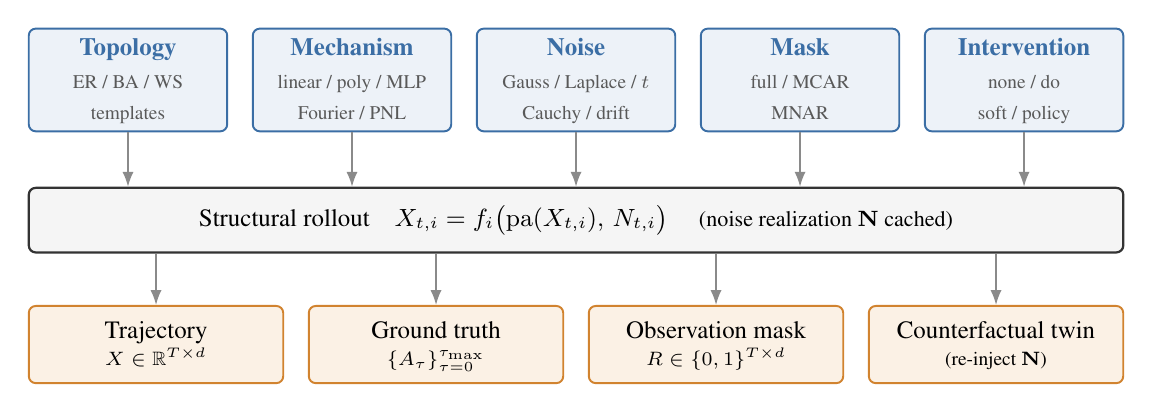
\begin{tikzpicture}[
  font=\small,
  axis/.style={draw=dtblue, line width=0.7pt, rounded corners=2.5pt,
               fill=dtbluefill, minimum width=2.52cm, minimum height=1.30cm,
               align=center, inner sep=2pt},
  outbox/.style={draw=dtorange, line width=0.7pt, rounded corners=2.5pt,
              fill=dtorangefill, minimum width=3.231cm, minimum height=0.98cm,
              align=center, inner sep=2pt},
  flow/.style={-{Latex[length=1.9mm]}, line width=0.6pt, dtgray}
]

% five configuration axes; the three rows share left and right edges
\node[axis] (ax0) at (1.260, 0)
  {{\bfseries\color{dtblue}\strut Topology}\\[1pt] \axsub{ER / BA / WS}\\ \axsub{templates}};
\node[axis] (ax1) at (4.105, 0)
  {{\bfseries\color{dtblue}\strut Mechanism}\\[1pt] \axsub{linear / poly / MLP}\\ \axsub{Fourier / PNL}};
\node[axis] (ax2) at (6.950, 0)
  {{\bfseries\color{dtblue}\strut Noise}\\[1pt] \axsub{Gauss / Laplace / $t$}\\ \axsub{Cauchy / drift}};
\node[axis] (ax3) at (9.795, 0)
  {{\bfseries\color{dtblue}\strut Mask}\\[1pt] \axsub{full / MCAR}\\ \axsub{MNAR}};
\node[axis] (ax4) at (12.640, 0)
  {{\bfseries\color{dtblue}\strut Intervention}\\[1pt] \axsub{none / do}\\ \axsub{soft / policy}};

% structural rollout, as wide as the axis row
\node[draw=dtink, line width=0.8pt, rounded corners=2.5pt, fill=black!4,
      minimum width=13.9cm, minimum height=0.82cm, align=center]
  (roll) at (6.95, -1.78)
  {\strut Structural rollout\quad
   $X_{t,i} = f_i\bigl(\mathrm{pa}(X_{t,i}),\, N_{t,i}\bigr)$
   \quad {\footnotesize(noise realization $\mathbf{N}$ cached)}};

\foreach \i in {0,...,4} {\draw[flow] (ax\i.south) -- (ax\i.south |- roll.north);}

% outputs, spanning the same width as the rows above
\node[outbox] (o0) at (1.616, -3.36)
  {\strut Trajectory\\[-1pt] {\scriptsize\strut $X \in \mathbb{R}^{T \times d}$}};
\node[outbox] (o1) at (5.172, -3.36)
  {\strut Ground truth\\[-1pt] {\scriptsize\strut $\{A_\tau\}_{\tau=0}^{\tau_{\max}}$}};
\node[outbox] (o2) at (8.728, -3.36)
  {\strut Observation mask\\[-1pt] {\scriptsize\strut $R \in \{0,1\}^{T \times d}$}};
\node[outbox] (o3) at (12.284, -3.36)
  {\strut Counterfactual twin\\[-1pt] {\scriptsize\strut (re-inject $\mathbf{N}$)}};

\foreach \i in {0,...,3} {\draw[flow] (o\i.north |- roll.south) -- (o\i.north);}

\end{tikzpicture}
\end{document}
